\documentclass{beamer}
\usepackage{graphicx}
\usepackage[utf8]{inputenc}
\usetheme{Warsaw}
\title[The Skein Hash Function Family]{A Brief Overview of\\the Skein Hash Function Family}
\author{Peter Boström}
\institute{Royal Institute of Technology (RIOT)}
\date{February 22, 2012}
\begin{document}

\begin{frame}
	\titlepage
\end{frame}

\begin{frame}{Skein -- Overview}
	Skein is built from these three new components:
	\vspace{4mm}
	\begin{itemize}
		\item Threefish
		\item Unique Block Iteration (UBI)
		\item Optional Argument System
	\end{itemize}
	\vspace{12mm}
	\begin{block}{Modular Design}
		``Dividing up our design makes Skein easier to understand, analyze, and prove properties about.''
	\end{block}
\end{frame}

\begin{frame}{Threefish}
	Tweakable block cipher, defined with a 256-, 512- and 1024-bit block size.
	\vspace{2mm}
	\begin{itemize}
		\item Design Philosophy
		\item Substitution-Permutation Network
		\item MIX function
		\item Tweakable Block Cipher
	\end{itemize}
\end{frame}

\begin{frame}{Threefish -- Design Philosophies}
	Skein and Threefish was designed with a few principles in mind:
	\vspace{2mm}
	\begin{itemize}
		\item Simplicity
		\item Security per clock cycle
		\item Maximum diffusion
		\item Flexibility
	\end{itemize}
\end{frame}

\begin{frame}{Threefish -- Substitution-Permutation Network}

	\begin{center}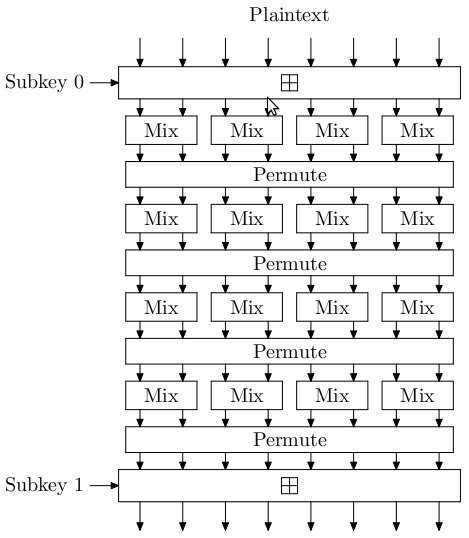
\includegraphics[width=100px]{skein-512}\end{center}

	A subkey is inject every 4 rounds, instead of each round. 72/80 rounds in total.

	\vspace{2mm}
	Threefish was designed to maximize diffusion, each input bit affects every output bit after 10 rounds.

	\vspace{2mm}
	But unlike a normal SP network Threefish doesn't use S-boxes..

\end{frame}

\begin{frame}{Threefish -- MIX function}

	\begin{center}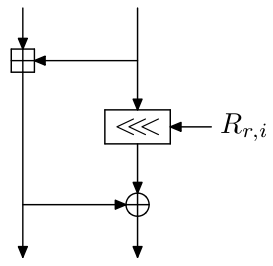
\includegraphics[width=90px]{mix}\end{center}

	Instead of S-boxes, Threefish has a really simple MIX function between two words consisting of a single ADD, rotation and XOR.

	\vspace{2mm}
	Threefish's non-linearity comes from mixing addition modulo $2^{64}$ and XOR.

\end{frame}

\begin{frame}{Threefish -- Tweakable Block Cipher}
	As a tweakable block cipher, Threefish takes a third input, a \emph{tweak} value, aside from plaintext/ciphertext and key.

	\vspace{2mm}
	Threefish's key schedule is generated from both the \emph{key} and \emph{tweak}, which together determine the permutation computed by the cipher.

	\vspace{2mm}
	\begin{block}{Tweak}
		``The purpose of the tweak is to make each block operation in Skein unique.''
	\end{block}
\end{frame}

\begin{frame}{Unique Block Iteration}

	\begin{center}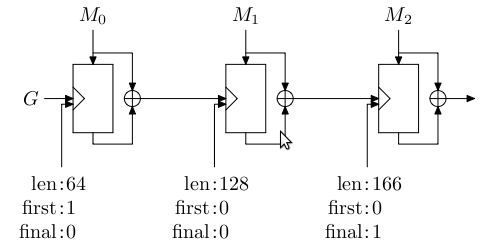
\includegraphics[width=120px]{ubi}\end{center}

	Unique Block Iteration (UBI) is a chaining mode which combines an input value (G) with an arbitrary-length input string to produce a fixed-size output.

	\vspace{2mm}
	The tweak value, encoding message type, length and first/final among others assures that each block is processed with a unique variant of the underlying cipher.

	\begin{block}{Tweak}
		``[A] message piece that produces one result in one location will produce a different result in a different location.''
	\end{block}

\end{frame}

\begin{frame}{Skein Hashing}

	\begin{center}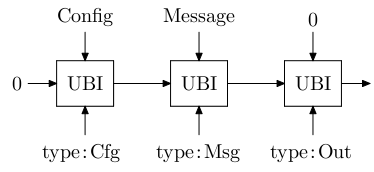
\includegraphics[width=120px]{skein-simple}\end{center}

	Skein is built on multiple invocations of UBI with different tweak values.

	\vspace{2mm}
	Regular Skein hashing is built from three UBI invocations:

	\vspace{2mm}
	\begin{itemize}
		\item Configuration [output length, tree-hashing parameters] (IV)
		\item Message
		\item Output transformation (Finalization)
	\end{itemize}
\end{frame}

\begin{frame}{Skein Hashing with Larger Output Size}

	\begin{center}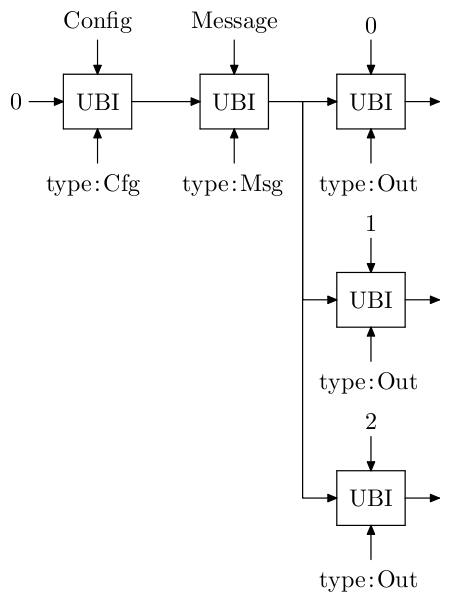
\includegraphics[width=140px]{skein-large}\end{center}

\end{frame}

\begin{frame}{Skein's Flexibility}

	\begin{center}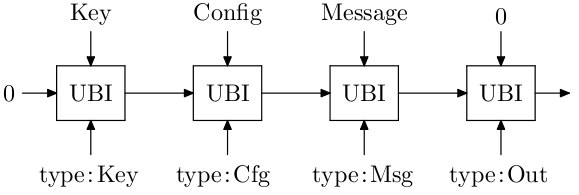
\includegraphics[width=140px]{skein-mac}\end{center}

	Skein's flexibility comes from its Optional-Argument System which defines support for using Skein as a/for:

	\vspace{2mm}
	\begin{itemize}
		\item Tree hashing
		\item Message Authentication Codes (MAC)
		\item Digital signatures
		\item Key-Derivation Function
		\item Pseudo-random number generator (PRNG)
		\item Stream cipher
	\end{itemize}

\end{frame}

\begin{frame}{The End}

	Thanks for listening!

\end{frame}

\end{document}
